\documentclass[tikz, border=5pt]{standalone}
\usepackage{tikz}
\usepackage{pgfplots}
\usepackage{pst-eucl}
\usepackage{tkz-euclide}

\begin{document}
  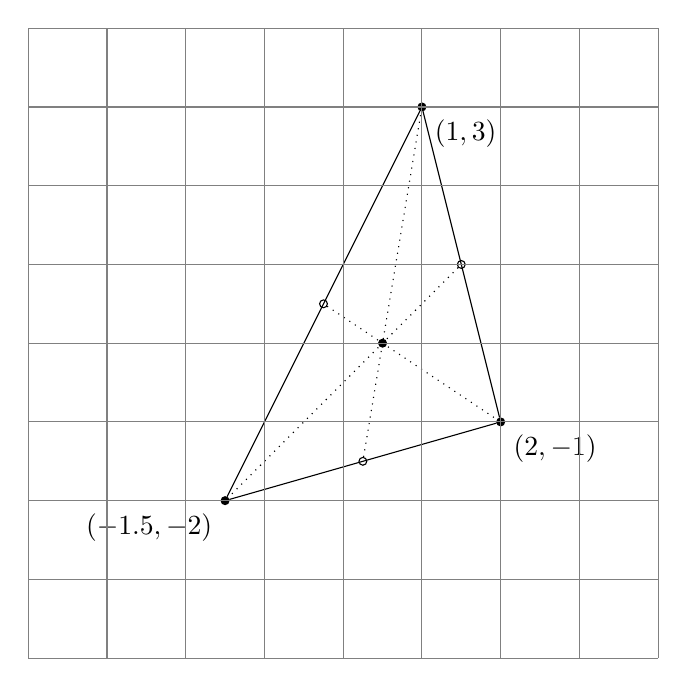
\begin{tikzpicture}
    \node[draw, circle, fill, inner sep = 1pt,label=below
    right:{$(1,3)$}] (a) at
    (1,3) {};
    \node[draw, circle, fill, inner sep = 1pt,label=below
    right:{$(2,-1)$}] (b) at
    (2,-1) {};
    \node[draw, circle, fill, inner sep = 1pt,label=below
    left:{$(-1.5,-2)$}] (c) at (-1.5,-2) {};
    \draw (a) -- (b) -- (c) -- (a);
    \node[draw, circle, inner sep = 1pt] (ab) at (1.5,1) {};
    \node[draw, circle, inner sep = 1pt] (bc) at (.25,-1.5) {};
    \node[draw, circle, inner sep = 1pt] (ca) at (-.25, .5) {};
    \node[draw, circle, fill, inner sep = 1pt] (centroid) at (.5,0)
    {};
    %\node[draw, circle, fill, inner sep = 1pt] (first_centroid) at
    %(2.25, 0) {};
    \draw[dotted] (ab) -- (c);
    \draw[dotted] (bc) -- (a);
    \draw[dotted] (ca) -- (b);
    %\draw[dashed] (a) -- (centroid);
    %\draw[dashed] (b) -- (centroid);
    %\draw[dashed] (c) -- (centroid);
    \tkzInit[xmax=4,ymax=4,xmin=-4,ymin=-4];
    \tkzGrid;
    \tkzAxeXY;
  \end{tikzpicture}
\end{document}
